% !TEX encoding = UTF-8 Unicode
\documentclass[
10pt,
aspectratio=169,
]{beamer}
\setbeamercovered{transparent=10}
\usetheme[
%  showheader,
%  red,
  purple,
%  gray,
%  graytitle,
  colorblocks,
%  noframetitlerule,
]{Verona}

\usepackage[T1]{fontenc}
\usepackage[utf8]{inputenc}
\usepackage{lipsum}
%%%%%%%%%%%%%%%%%%%%%%%%%%%%%%%
% Mac上使用如下命令声明隶书字体,windows也有相关方式,大家可自行修改
%\providecommand{\lishu}{\CJKfamily{zhli}}
%%%%%%%%%%%%%%%%%%%%%%%%%%%%%%%
\usepackage{tikz}
\usetikzlibrary{fadings}
\usetikzlibrary{shapes.geometric}
\usetikzlibrary{positioning}
%\tikzset{
%  every overlay node/.style={
%    draw=black,fill=white,rounded corners,anchor=south west,
%  },
%}
% Usage:
% \tikzoverlay at (-1cm,-5cm) {content};
% or
% \tikzoverlay[text width=5cm] at (-1cm,-5cm) {content};
%\def\tikzoverlay{%
%   \tikz[baseline,overlay]\node[every overlay node]
%}%
\tikzset{
  every overlay node/.style={
    anchor=north west,
  },
}
\def\tikzoverlay{%
   \tikz[baseline,overlay]\node[every overlay node]
}%


\newenvironment{smallgreentext}{\scriptsize\color{green}}{\par}
\newenvironment{smallbluetext}{\scriptsize\color{blue}}{\par}

%
%\setbeamertemplate{sections/subsections in toc}[ball]
%\usepackage{xeCJK}
\usepackage{adjustbox} % Shrink stuff
\usepackage{listings}
\usepackage{caption}
\usepackage{subcaption}
\usefonttheme{professionalfonts}
\def\mathfamilydefault{\rmdefault}
\usepackage{amsmath}
\usepackage{multirow}
\usepackage{booktabs}
\usepackage{bm}
\setbeamertemplate{section in toc}{\hspace*{1em}\inserttocsectionnumber.~\inserttocsection\par}
\setbeamertemplate{subsection in toc}{\hspace*{2em}\inserttocsectionnumber.\inserttocsubsectionnumber.~\inserttocsubsection\par}
\setbeamerfont{subsection in toc}{size=\small}
\AtBeginSection[]{%
	\begin{frame}%
		\frametitle{Outline}%
		\textbf{\tableofcontents[currentsection]} %
	\end{frame}%
}

\AtBeginSubsection[]{%
	\begin{frame}%
		\frametitle{Outline}%
		\textbf{\tableofcontents[currentsection, currentsubsection]} %
	\end{frame}%
}

\title{Introducci\'on: Justificaci\'on}
\subtitle{Estructuraci\'on y realizaci\'on de la propuesta}
\author[L.M.]{Luis Alejandro Morales, Ph.D.}
\mail{lmoralesm@unal.edu.co}
\institute[UNAL]{Facultad de Ingenier\'ia, Departamento de Ingnenier\'ia Civil y Agr\'icola\\
Universidad Nacional de Colombia, Bogot\'a}
\date{\today}
\titlegraphic[width=3cm]{logo_01u}{}

%%%%%%%%%%%%%%%%%%%%%%%%%%%%%%%%
% ----------- 标题页 ------------
%%%%%%%%%%%%%%%%%%%%%%%%%%%%%%%%
% New commands
\newcommand{\gi}{\texttt{Git}}
\newcommand{\gih}{\texttt{GitHub}}
\newcommand{\co}[1]{\alert{\textbf{\large \texttt{#1}}}}
\begin{document}



\maketitle

%%% define code
\defverbatim[colored]\lstI{
	\begin{lstlisting}[language=C++,basicstyle=\ttfamily,keywordstyle=\color{red}]
	int main() {
	// Define variables at the beginning
	// of the block, as in C:
	CStash intStash, stringStash;
	int i;
	char* cp;
	ifstream in;
	string line;
	[...]
	\end{lstlisting}
}
%%%%%%%%%%%%%%%%%%%%%%%%%%%%%%%%
% ----------- FRAME ------------
%%%%%%%%%%%%%%%%%%%%%%%%%%%%%%%%

%---
\section{Introducci\'on}
\begin{frame}[c]{Partes de la introducci\'on}
\begin{enumerate}
\item La justificaci\'on: Texto que justifica, con base en unos antecedentes (revisi\'on bibliogr\'afica), una hip\'otesis, argumento, pregunta de investigaci\'on.
\item Hip\'otesis: Es una declaraci\'on en donde se introduce al lector de una forma l\'ogica y concisa acerca de lo que trata la investigaci\'on. 
\end{enumerate}

\end{frame}

\begin{frame}{Introducci\'on: The topdown approach}
\tikzoverlay[text width=1.5cm] at (2.3cm,2cm) {
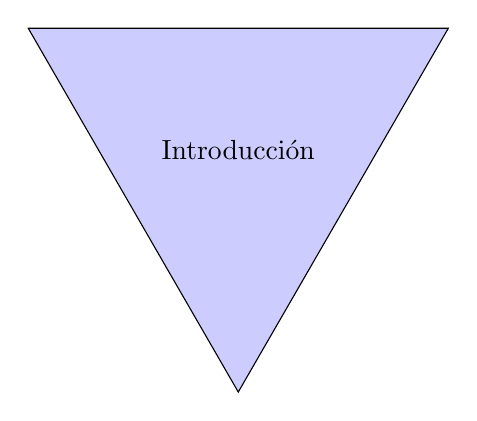
\begin{tikzpicture} 
% \node[regular polygon,regular polygon sides=3, draw, fill=blue!20, shape border rotate=180] at (-4cm,0){Introducci\'on};
 \node[regular polygon,regular polygon sides=3, draw, fill=blue!20, shape border rotate=180] at (current page.center){Introducci\'on};
\end{tikzpicture}
};
\tikzoverlay[text width=4.5cm] at (8.3cm,2cm) {
\alert{What is the status quo?}
};
\tikzoverlay[text width=4.5cm] at (8.3cm,0cm) {
\alert{What is wrong with the status quo?}
};
\tikzoverlay[text width=4.5cm] at (8.3cm,-2cm) {
\alert{How does my project/paper go beyond the status quo?}
};
\end{frame}

%---
\section{Justificaci\'on}
\begin{frame}{Justificaci\'on}
\begin{itemize}
\item Establece el porque la investigazci\'on o trabajo de grado es relevante.
\item Indica los autores, personajes, casos de estudio, involucrados en la investigaci\'on.
\item En concreto, hace referencia a casos directamente relacionados con la investigaci\'on.
\item Determina porque la realizaci\'on de esa investigaci\'on cambia o complementa lo ya existente. 
\end{itemize}
\end{frame}

\begin{frame}{Ejercicio}
Lea la introducci\'on de un  art\'iculo de inter\'es y determine la justificaci\'on y/o la motivaci\'on de la investigaci\'on.
\end{frame}


\end{document}


